% \chapter{Introduction}
% \label{chap:introduction}

% \noindent
% \begin{minipage}[c]{0.55\textwidth}
% Chest X-ray (CXR) images are fundamental diagnostic tools used to identify various lung diseases. They provide a non-invasive means for clinicians to visualize the internal structures of the chest, facilitating the detection of abnormalities such as infections, tumors, or chronic respiratory conditions. This imaging modality remains a cornerstone of clinical practice due to its accessibility and effectiveness.
% \end{minipage}
% \hfill
% \begin{minipage}[c]{0.4\textwidth}
% \centering
% 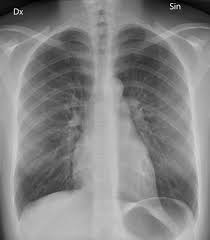
\includegraphics[width=\textwidth]{images/cxr_sample}
% \captionof{figure}{A sample chest X-ray image.}
% \label{fig:cxr_sample}
% \end{minipage}

% \section{Existing CXR Image Datasets}
% % Add your text here regarding datasets like ChestX-ray14, MIMIC-CXR, or CheXpert.

% \section{Need for Synthetic CXR}
% % Add your text here about why data augmentation or privacy-preserving synthetic data is needed.

% \subsection{Metrics}
% Frechet Inception Distance (FID) is the standard metric used to evaluate the quality of generated images. 
% % As a baseline FID score between Normal (pathology free) and Abnormal (Pathology contained) x-ray images is 
% % measured to check how good are later FIDs compared to this baseline.

% % FID between Normal and Abnormal images is: 19.31

\chapter{Introduction}
\label{chap:introduction}


Chest X-ray (CXR) images are some of the most widely used diagnostic tools in modern medicine for the detection and monitoring of thoracic diseases. 
It provides a fast and cost-effective method for visualizing internal structures such as the lungs, heart, and surrounding tissues. 
Radiologists rely heavily on CXR images to diagnose conditions including pneumonia, tuberculosis, lung cancer, and other chronic respiratory disorders.

Despite its widespread use, interpretation of CXR images requires significant expertise, as subtle variations in intensity and structure can 
correspond to clinically relevant findings. With the rise of deep learning, artificial systems have been developed to assist radiologists in 
detecting abnormalities, thereby improving diagnostic efficiency and reducing time to diagnose.

These systems could be very helpful in resource-constrained regions and also in pandemic times. The main challenges in training these artificial models are: 
1) scarcity of publicly available data, and 
2) high imbalance across pathologies. 

To address this issue, synthetic Chest X-ray image generation methods have been proposed. 
While these works provide models to generate synthetic data, we observed them to be ineffective in classification tasks \cite{andrewng_paper}. \textcolor{red}{What classification task?}.

In this work, we first tried simple fine-tuning of GANs and diffusion models using disease labels as prompts, which did not give good performance. \textcolor{red}{What do you mean by not good performacnce?}
Finding that CLIP embeddings of disease labels were a possible culprit, we tried complete descriptions of images as conditioning \cite{}, 
but this also failed to generate images aligned with prompts.  

To verified our results we used RadGraph to extract entities from generated images and checked if disease mentioned in the prompt is present in it.
Apart from that we used mdclip to compare the generated image embeddings with prompt used for generating and also "Normal" , and found out that 
most images generated are as close to normal as to the prompt used to generate it \textcolor{red}{this is good.. please elaborate}.

When it comes to classification there is not much improvement in performance of models when synthetic data is used \textcolor{red}{pls elaborate}.


\begin{figure}[h!]
\centering
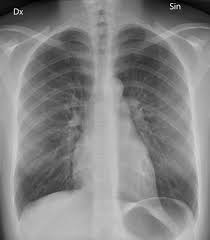
\includegraphics[width=0.5\textwidth]{images/cxr_sample}
\caption{A sample chest X-ray image.}
\label{fig:cxr_sample}
\end{figure}


\section{Existing CXR Image Datasets}

The success of deep learning models in medical imaging is strongly dependent on the availability of large-scale annotated datasets. Several publicly available CXR datasets have been introduced to facilitate research:

\section{CXR Datasets Overview}

Several large-scale chest X-ray datasets have been developed to support deep learning research. The most widely used among them are NIH ChestX-ray14, CheXpert, and MIMIC-CXR. These datasets differ in scale, labeling quality, and availability of associated radiology reports.

\subsection{Dataset Comparison}

\begin{table}[h]
\centering
\begin{tabular}{lccccc}
\hline
\textbf{Dataset} & \textbf{Train} & \textbf{Validation} & \textbf{Test} & \textbf{Labels} & \textbf{Reports} \\
\hline
NIH  & 86K & 6K & 6K & Yes (noisy) & No \\
CheXpert         & 224K & 5K & 500 & Yes (uncertain) & No \\
MIMIC-CXR        & 367k & 3k & 5k & Yes & Yes \\
\hline
\end{tabular}
\caption{Comparison of major CXR datasets. Counts are approximate and depend on preprocessing and splits.}
\label{tab:cxr_datasets}
\end{table}

\subsection{NIH}

NIH \cite{filice2020crowdsourcing} dataset is one of the earliest large-scale publicly available CXR datasets, containing over 120,000 
frontal-view X-ray images from more than 30,000 patients. It includes annotations for 14 disease classes such 
as pneumonia, atelectasis, and cardiomegaly.

\begin{table}[h!]
\centering
\caption{Distribution of pathology labels in the NIH Chest X-ray dataset}
\label{tab:nih_distribution}
\begin{tabular}{lcc}
\hline
\textbf{Pathology Label} & \textbf{Percentage} & \textbf{Count} \\
\hline
No Finding & 53.84\% & 60,361 \\
Atelectasis & 10.31\% & 11,559 \\
Cardiomegaly & 2.48\% & 2,776 \\
Effusion & 11.88\% & 13,317 \\
Infiltration & 17.74\% & 19,894 \\
Mass & 5.16\% & 5,782 \\
Nodule & 5.65\% & 6,331 \\
Pneumonia & 1.28\% & 1,431 \\
Pneumothorax & 4.73\% & 5,302 \\
Consolidation & 4.16\% & 4,667 \\
Edema & 2.05\% & 2,303 \\
Emphysema & 2.24\% & 2,516 \\
Fibrosis & 1.50\% & 1,686 \\
Pleural Thickening & 3.02\% & 3,385 \\
Hernia & 0.20\% & 227 \\
\hline
\end{tabular}
\end{table}


\subsection{CheXpert}

CheXpert \cite{Irvin2019} is a large-scale dataset developed by Stanford University, consisting of over 220,000 chest X-ray images. It improves upon NIH ChestX-ray14 by introducing a more robust label extraction pipeline that explicitly models \textit{uncertainty} in annotations.
Each label can take values such as positive, negative, or uncertain, allowing researchers to experiment with different uncertainty handling strategies. However, similar to NIH ChestX-ray14, the full radiology reports are not publicly released.
CheXpert also provides a small, high-quality validation and test set annotated by radiologists, making it a strong benchmark for model evaluation.
\cite{chexpert_dataset}
\begin{table}[h!]
\centering
\caption{Pathological Distribution of images in chexpert}
\label{tab:chexpert_distribution}
\begin{tabular}{lccc}
\hline
\textbf{Pathology} & \textbf{Positive (\%)} & \textbf{Uncertain (\%)} & \textbf{Negative (\%)} \\
\hline
No Finding & 16627 (8.86) & 0 (0.0) & 171014 (91.14) \\
Enlarged Cardiomediastinum & 9020 (4.81) & 10148 (5.41) & 168473 (89.78) \\
Cardiomegaly & 23002 (12.26) & 6597 (3.52) & 158042 (84.23) \\
Lung Lesion & 6856 (3.65) & 1071 (0.57) & 179714 (95.78) \\
Lung Opacity & 92669 (49.39) & 4341 (2.31) & 90631 (48.30) \\
Edema & 48905 (26.06) & 11571 (6.17) & 127165 (67.77) \\
Consolidation & 12730 (6.78) & 23976 (12.78) & 150935 (80.44) \\
Pneumonia & 4576 (2.44) & 15658 (8.34) & 167407 (89.22) \\
Atelectasis & 29333 (15.63) & 29377 (15.66) & 128931 (68.71) \\
Pneumothorax & 17313 (9.23) & 2663 (1.42) & 167665 (89.35) \\
Pleural Effusion & 75696 (40.34) & 9419 (5.02) & 102526 (54.64) \\
Pleural Other & 2441 (1.30) & 1771 (0.94) & 183429 (97.76) \\
Fracture & 7270 (3.87) & 484 (0.26) & 179887 (95.87) \\
Support Devices & 105831 (56.40) & 898 (0.48) & 80912 (43.12) \\
\hline
\end{tabular}
\end{table}
\subsection{MIMIC-CXR}

MIMIC-CXR \cite{Johnson2019} is one of the largest and most comprehensive CXR datasets, containing over 375,000 images associated with more than 
200,000 studies. It is derived from clinical data collected at Beth Israel Deaconess Medical Center. \cite{mimic_cxr}
A key advantage of MIMIC-CXR is the availability of corresponding radiology reports for each image, enabling multimodal learning 
and report generation tasks. Labels are often derived using tools such as CheXpert labeler, but raw reports allow for more flexible 
and accurate annotation strategies. Unlike NIH and CheXpert, standard train-validation-test splits are not strictly defined and are 
often created by researchers based on patient-level separation.


\begin{table}[h!]
\centering
\caption{Distribution of pathology labels in the MIMIC-CXR dataset}
\label{tab:mimic_distribution}
\begin{tabular}{lccc}
\hline
\textbf{Disease} & \textbf{Number of Images} & \textbf{Percentage (\%)} \\
\hline
No Finding & 141239 & 22.85 \\
Support Devices & 81890 & 13.25 \\
Pleural Effusion & 74745 & 12.09 \\
Lung Opacity & 74302 & 12.02 \\
Atelectasis & 63485 & 10.27 \\
Cardiomegaly & 62554 & 10.12 \\
Edema & 35279 & 5.71 \\
Pneumonia & 25489 & 4.12 \\
Consolidation & 14236 & 2.30 \\
Pneumothorax & 14001 & 2.26 \\
Lung Lesion & 10490 & 1.70 \\
Enlarged Cardiomediastinum & 9752 & 1.58 \\
Fracture & 7404 & 1.20 \\
Pleural Other & 3319 & 0.54 \\
\hline
\end{tabular}
\end{table}


\begin{figure}[ht]
    \centering
    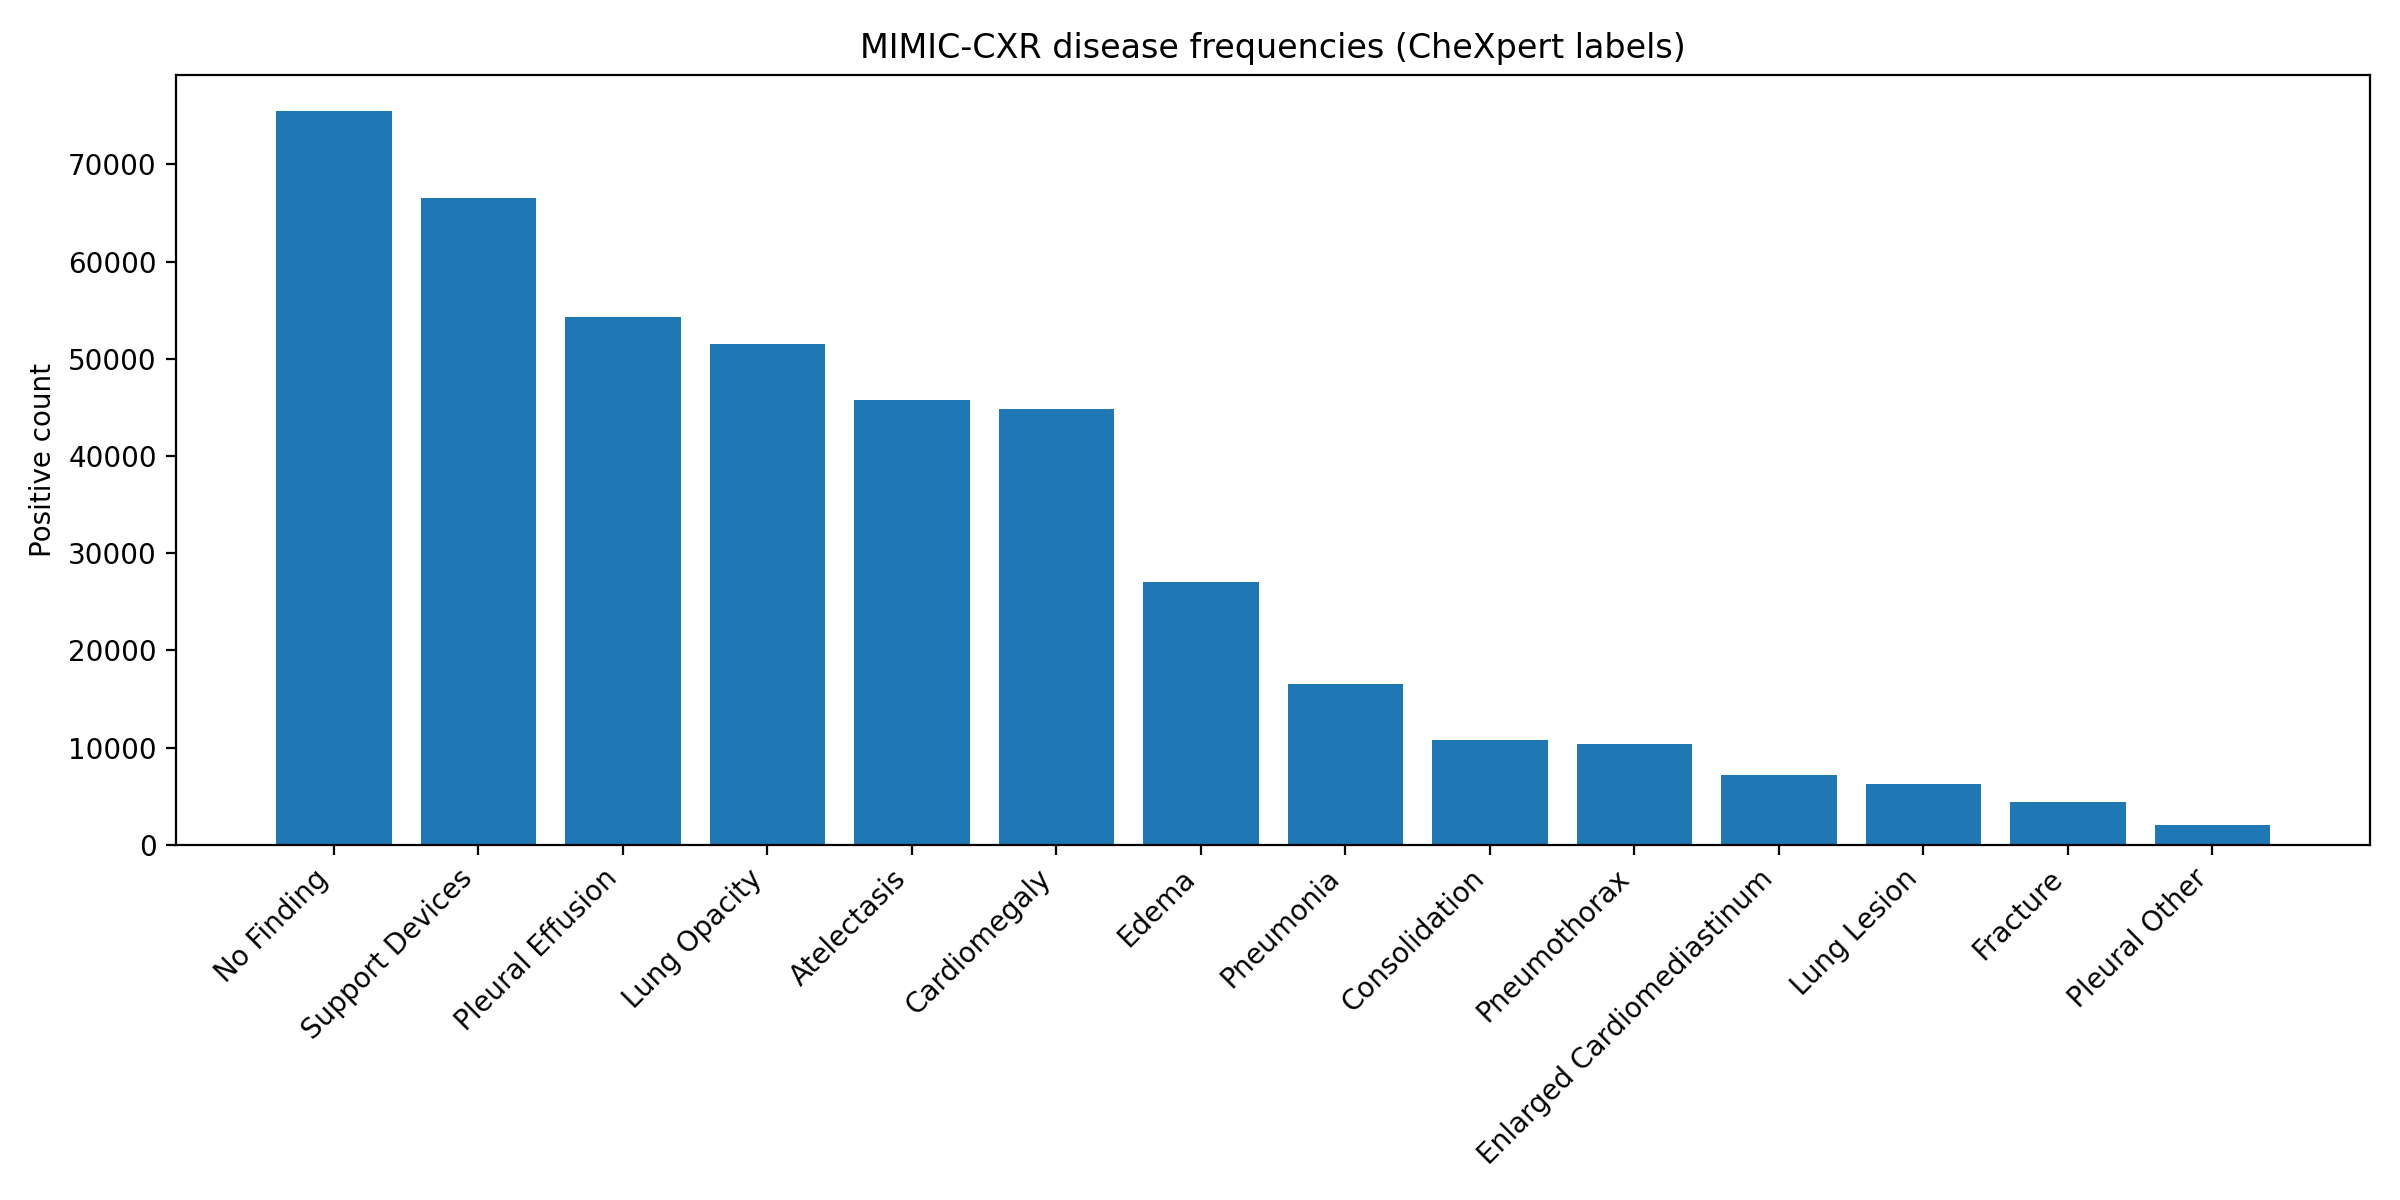
\includegraphics[width=0.75\textwidth]{images/mimic_imbalance.png}
    \caption{Example of class imbalance in MIMIC-CXR dataset.}
    \label{fig:class_imbalance}
\end{figure}


\section{Need for Synthetic CXR}

The generation of synthetic CXR images has emerged as a promising solution to address the limitations of real-world datasets. There are several key motivations:

\begin{itemize}
    \item \textbf{Data Scarcity}: Certain pathological conditions are rare, leading to insufficient training samples. Generative models can augment such underrepresented classes.
    
    \item \textbf{Privacy Preservation}: Medical data is highly sensitive and often restricted. Synthetic data allows sharing without exposing patient information.
    
    \item \textbf{Class Imbalance}: Many datasets are dominated by normal cases. Synthetic generation can help balance datasets and improve model robustness.
    
    \item \textbf{Controlled Generation}: Generative models enable conditional synthesis \cite{Chambon2022RoentGen}, allowing the creation of images with specific 
    pathologies or attributes. They even enables editing given CXR images \cite{perez-garcia_bond-taylor_radedit}, like visualizing how the same infected CXR looks without that disease
    or vice versa
\end{itemize}

Recent advances in generative modeling, particularly diffusion models and GANs, have demonstrated strong capabilities 
in producing high-fidelity medical images \cite{chambon2024roentgen,Weber2023Cheff,perez-garcia_bond-taylor_radedit}, 
making them suitable for CXR synthesis. 





% ---------------
%  FID
% ---------------


% Example baseline (optional)
% FID between Normal and Abnormal images is: 19.31